\documentclass[11pt,spanish]{article} % Tipo y tamaño de letra del documento.


\usepackage[utf8]{inputenc}
\usepackage{subfiles}
\usepackage{biblatex}
\addbibresource{references.bib}
\usepackage{multicol}
\usepackage{amsfonts}
\usepackage{blindtext}
\usepackage{mathrsfs}
\usepackage{amsmath}
\usepackage{siunitx}
\usepackage{centernot}
\usepackage[shortlabels]{enumitem}
\usepackage{subfig}
\usepackage{datetime}
\usepackage{listingsutf8}
\usepackage[spanish]{babel}
\usepackage{tikz}
\usepackage{hyperref}
\usepackage[vlined,ruled,linesnumbered]{algorithm2e}
\usepackage{listings}
%\usepackage{float}
\usepackage{url}
\usepackage{csquotes}
\usepackage{fourier} %font
\usepackage[top=2cm, bottom=2cm, left=2.5cm, right=2.5cm]{geometry}
\usepackage{pgfplots}
\usepackage{fancyhdr}
\usepackage{mdframed}
\usepackage{tikzducks}
\usepackage[nameinlink]{cleveref}
\usepackage{epigraph} 

\pgfplotsset{compat=1.18}

\usetikzlibrary{shapes.arrows, shapes.geometric, arrows.meta,angles,quotes,positioning,arrows,fit,quotes,calc}
\tikzset{>=latex} 


\Crefname{figure}{Fig.}{Figs.}
\newcommand\crefrangeconjunction{--}
\Crefname{table}{Tabla}{Tablas}
\Crefname{subsubsection}{Subsubsec.}{Subsubsections}
\Crefname{subsection}{Subsec.}{Subsections}
\Crefname{section}{Sec.}{Sections}
\Crefname{equation}{eq.}{eqs.}
\crefname{thm}{Theorem}{theorems}
\Crefname{thm}{Theorem}{Theorems} 

\definecolor{algoco}{rgb}{0,0.44,1}

\hypersetup{
  colorlinks=true,
  linkcolor=algoco,
  citecolor=blue,
  urlcolor=blue,
}

\lstset{
extendedchars=true
inputencoding=utf8/latin1,
basicstyle=\footnotesize\sffamily\color{black},
commentstyle=\slshape \color{gray},
numbers=left,
numbersep=10pt,
numberstyle=\tiny\color{red!80!black},
keywordstyle=\color{red!80!magenta},
showspaces=false,
showstringspaces=false,
stringstyle=\color{cyan!80!black},
tabsize=2,
literate={á}{{\'a}}1 {é}{{\'e}}1 {í}{{\'i}}1 {ó}{{\'o}}1 {ú}{{\'u}}1,
frame = single, 
numbers = none,
float, floatplacement = ht, captionpos = b,
xleftmargin = 2em, xrightmargin = 2em, 
}

\newcommand{\ub}[1]{\underbrace{#1}}
\newcommand\tcm{\textcolor{magenta}}
\newcommand\tca{\textcolor{algoco}}
 

\newcommand{\tnum}{2} % reemplace 2 por el número de la tarea
\newcommand{\sem}{2024-2} % reemplace 2024-2 por el semestre correspondiente
\newcommand{\campus}{Casa Central \\ Valparaíso} % reemplace Casa Central por el campus correspondiente
\newcommand{\rolusm}{2025073100-1} % reemplace 2025073100-1 por su rol
\newcommand{\namestudent}{Al Goritmo Pérez} % reemplace Al Goritmo Pérez por su nombre

\headheight=14pt
\linespread{1.3}
\author{\namestudent}
\pagestyle{fancy}
\fancyhf{}%
\fancyfoot[R]{ \namestudent \\ \rolusm}
\fancyfoot[L]{Campus \campus} 
\fancyfoot[C]{\thepage}
\rhead{2024-2}
\lhead{INF-221}
\renewcommand{\headrulewidth}{0.4pt}
\renewcommand{\footrulewidth}{0.4pt}
\newbool{programs}
\boolfalse{programs}
\chead{REPORTE TAREA \tnum~}



\title{
  \huge
  \textbf{REPORTE TAREA \tnum~ \\ ALGORITMOS Y COMPLEJIDAD} \\[1ex]
  \emph{\textquote{Explorando la Distancia entre Cadenas, una Operación a la Vez}}
  }

  
\date{
  \small
  \today\\
  \currenttime
}




\begin{document}
\maketitle
\thispagestyle{fancy} 
\vspace{-1.0\baselineskip}




\begin{abstract}
  \textit{ 
    Un resumen es un breve compendio que sintetiza todas las secciones clave de un trabajo de investigación: la introducción, los objetivos, la infraestructura y métodos, los resultados y la conclusión. Su objetivo es ofrecer una visión general del estudio, destacando la novedad o relevancia del mismo, y en algunos casos, plantear preguntas para futuras investigaciones. El resumen debe cubrir todos los aspectos importantes del estudio para que el lector pueda decidir rápidamente si el artículo es de su interés.

En términos simples, el resumen es como el menú de un restaurante que ofrece una descripción general de todos los platos disponibles. Al leerlo, el lector puede hacerse una idea de lo que el trabajo de investigación tiene para ofrecer \cite{elsevier_abstract_2024}.

\textbf{La extensión del resumen, para esta entrega, debe ser tal que la totalidad del índice siga apareciendo en la primera página. Recuerde que NO puede modificar el tamaño de letra, interlineado, márgenes, etc.}

  }
     
\end{abstract}

\setcounter{tocdepth}{1}
\tableofcontents


\newpage
\section{Introducción}
\begin{mdframed}
    \textbf{La extensión máxima para esta sección es de 2 páginas.}
\end{mdframed}

La introducción de este tipo de informes o reportes, tiene como objetivo principal \textbf{contextualizar el problema que se va a analizar}, proporcionando al lector la información necesaria para entender la relevancia del mismo. 

Es fundamental que en esta sección se presenten los antecedentes del problema, destacando investigaciones previas o principios teóricos que sirvan como base para los análisis posteriores. Además, deben explicarse los objetivos del informe, que pueden incluir la evaluación de un algoritmo, la comparación de métodos o la validación de resultados experimentales.

Aunque la estructura y el enfoque siguen principios de trabajos académicos, se debe recordar que estos informes no son publicaciones científicas formales, sino trabajos de pregrado. Por lo tanto, se busca un enfoque claro y directo, que permita al lector comprender la naturaleza del problema y los objetivos del análisis, sin entrar en detalles excesivos. 


Introduction Checklist de \citetitle{GoodScientificPaper} \cite{GoodScientificPaper}, adaptada a nuestro contexto:

\begin{itemize}
\item Indique el \textbf{campo del trabajo} (Análisis y Diseño de algoritmos en Ciencias de la Computación), por qué este campo es importante y qué se ha hecho ya en este área, con las \textbf{citas} adecuadas de la literatura académica o fuentes relevantes.
\item Identifique una \textbf{brecha} en el conocimiento, un desafío práctico, o plantee una \textbf{pregunta} relacionada con la eficiencia, complejidad o aplicabilidad de un algoritmo particular.
\item Resuma el propósito del informe e introduzca el análisis o experimento, dejando claro qué se está investigando o comparando, e indique \textbf{qué es novedoso} o por qué es significativo en el contexto de un curso de pregrado.
\item Evite; repetir el resumen; proporcionar información innecesaria o fuera del alcance de la materia (limítese al análisis de algoritmos o conceptos de complejidad); exagerar la importancia del trabajo (recuerde que se trata de un informe de pregrado); afirmar novedad sin una comparación adecuada con lo enseñado en clase o la bibliografía recomendada.
\end{itemize}



\begin{mdframed}
Recuerde que este es su trabajo, y sólo usted puede expresar con precisión lo que ha aprendido y quiere transmitir. Si lo hace bien, su introducción será más significativa y valiosa que cualquier texto automatizado. ¡Confíe en sus habilidades, y verá que puede hacer un mejor trabajo que cualquier herramienta que automatiza la generación de texto!
\end{mdframed}



\newpage
\section{Diseño de Algoritmos} 
\input{sections/design}

\newpage
\section{Implementaciones}
\begin{mdframed}
    \textbf{La extensión máxima para esta sección es de 1 página.}
\end{mdframed}

Aquí deben explicar la estructura de sus programas haciendo referencias a los archivos y funciones de su entrega. No adjunte código en esta sección.
\begin{mdframed}
    Si se utiliza algún código, idea, o contenido extraído de otra fuente, este \textbf{debe} ser citado en el lugar exacto donde se utilice, en lugar de mencionarlo al final del informe.\\
\end{mdframed}

\newpage
\section{Experimentos}
\begin{mdframed}
    \textbf{La extensión máxima para esta sección es de 6 página.}
\end{mdframed}


\epigraph{``\textit{Non-reproducible single occurrences are of no significance to
science.}''}{---\citeauthor{popper2005logic},\citeyear{popper2005logic} \cite{popper2005logic}}
En la sección de Experimentos, es fundamental detallar la infraestructura utilizada para asegurar la reproducibilidad de los resultados, un principio clave en cualquier experimento científico. Esto implica especificar tanto el hardware (por ejemplo, procesador Intel Core i7-9700K, 3.6 GHz, 16 GB RAM DDR4, almacenamiento SSD NVMe) como el entorno software (sistema operativo Ubuntu 20.04 LTS, compilador g++ 9.3.0, y cualquier librería relevante). Además, se debe incluir una descripción clara de las condiciones de entrada, los parámetros utilizados y los resultados obtenidos, tales como tiempos de ejecución y consumo de memoria, que permitan a otros replicar los experimentos en entornos similares. \textit{La replicabilidad es un aspecto crítico para validar los resultados en la investigación científica computacional} \cite{inbookFonseca}.

\subsection{Dataset (casos de prueba)}
\begin{mdframed}
    \textbf{La extensión máxima para esta sección es de 2 páginas.}
\end{mdframed}


\subsection{Resultados}
\begin{mdframed}
    \textbf{La extensión máxima para esta sección es de 4 páginas.}
\end{mdframed}


En esta sección, los resultados obtenidos, como las gráficas o tablas, deben estar respaldados por los datos generados durante la ejecución de sus programas. Es fundamental que, junto con el informe, se adjunten los archivos que contienen dichos datos para permitir su verificación. Además, se debe permitir y especficiar como obtener esos archivos desde una ejecución en otro computador (otra infraestructura para hacer lso experimentos).

\textbf{No es necesario automatizar la generación de las gráficas}, pero sí es imprescindible que se pueda confirmar que las visualizaciones presentadas son producto de los datos generados por sus algoritmos, aunque la trazabilidad de los datos hasta las visualizaciones es esencial para garantizar que su validez: describa cómo se generaron los datos, cómo se procesaron y cómo se visualizaron de manera que pueda ser replicado por quien lea su informe.

Agregue gráficas que muestren los resultados de sus experimentos. La cantidad de páginas es limitada, por lo tanto escoja las gráficas más representativas y que muestren de manera clara los resultados obtenidos. Esta elección es parte de lo que se evaluara en la sección de presentación de resultados. Referencie las figuras en el texto, describa lo que se observa en ellas y por qué son relevantes.

En la \cref{fig:scatterplot_1} se muestra un scatterplot hecho con \href{https://es.overleaf.com/learn/latex/TikZ_package}{TikZ} con el tamaño ideal cuando se incluyen dos figuras. Queda a criterio de usted el decidir qué figuras incluir.

\begin{figure}[H]
    \centering
    
\begin{tikzpicture}
    %\begin{loglogaxis}[
    %\begin{semilogxaxis}[ % Cambiar a semilogxaxis    
    \begin{axis}[
        xlabel={Número de Cudastreams },
        ylabel={Tiempo [ms]},
        grid=major,
        legend pos=north west,
        legend cell align={left},
        width=16cm,
        height=10cm, 
        xtick=data,
    ]
    \addplot[blue, only marks, mark=square*] coordinates {
        (2   , 14.229344)
        (4   , 13.435616 )
        (8   , 12.929280 )
        (12  , 12.628000 )
        (16  , 13.286176 )
        (20  , 13.873152 )
        (24  , 13.531168 )
        (28  , 14.116384 )
        (32  , 14.518528 )
        (36  , 14.448992 )
        (40  , 14.356640 )
        (44  , 15.226560 )
        (48  , 14.473888 )
        (52  , 15.066720 )
        (56  , 15.426560 )
        (60  , 15.380416 )
        (64  , 15.348064 )
    };
    \addlegendentry{GPU\_51 (1)}
    \addplot[red, only marks, mark=square*] coordinates {
        (2  , 12.799264 ) 
        (4  , 12.956192 )
        (8  , 13.371104 )
        (12 , 14.495616 )
        (16 , 14.783360 ) 
        (20 , 15.152672 ) 
        (24 , 15.475488 ) 
        (28 , 15.676416 ) 
        (32 , 15.948800 ) 
        (36 , 16.064129 ) 
        (40 , 15.904544 ) 
        (44 , 16.157921 ) 
        (48 , 16.444992 ) 
        (52 , 16.943169 ) 
        (56 , 16.894304 ) 
        (60 , 17.689600 ) 
        (64 , 17.559551 ) 
    };
    \addlegendentry{GPU\_6 (2)}
    \addplot[green, only marks, mark=square*] coordinates {
        (6, 17.607168) 
        (12, 12.159264) 
        (24, 12.239648) 
        (24, 12.169376) 
        (48, 12.490624) 
        (72, 14.081920) 
    };
    \addlegendentry{GPU\_7 (3)}
   
\end{axis}
%\end{semilogxaxis} % Cambiar a semilogxaxis
\end{tikzpicture}

    \caption{Ejemplo de scatterplot hecho con tikz. Tamaño ideal 1.}
    \label{fig:scatterplot_1}
\end{figure}


\begin{figure}[H]
    \centering
    \begin{minipage}[t]{0.5\textwidth}
    \begin{tikzpicture}[scale=0.7]
    %\begin{loglogaxis}[
    %\begin{semilogxaxis}[ % Cambiar a semilogxaxis    
    \begin{axis}[
        xlabel={\Large Meandistance [\AA] },
        ylabel={\Large Efree [eV]},
        %grid=major,
        legend pos=north east,
        legend cell align={left},
        %log basis x=10,
        %log basis y=10,
        %xmin=2, xmax=2^21,
        %ymin=0.1, ymax=100,
        width=10cm, % Ajusta el ancho de la gráfica
        height=10cm, % Ajusta la altura de la gráfica
        %xtick=data,
    ]
    \addplot[magenta , only marks, mark=square*, mark options={draw=black,line width = 1pt}, mark size=4pt] coordinates {
        %(7.112914 ,	-255.554964)
        (5.807670 ,	-255.571675)
        (2.903835 ,	-255.534455)
        (5.029590 ,	-255.564079)
        (4.106643 ,	-255.551738)       
        };
    \addlegendentry{cantmax = 0} 
    \addplot[cyan , only marks, mark=square*, mark options={draw=black,line width = 1pt}, mark size=4pt] coordinates {
        (7.112914 ,	-255.554964)   
        };
        \addlegendentry{cantmax = 1} 
\end{axis}
%\end{semilogxaxis} % Cambiar a semilogxaxis
\end{tikzpicture}
    \end{minipage}%
    \begin{minipage}[t]{0.5\textwidth}
    \begin{tikzpicture}[scale=0.7]
    %\begin{loglogaxis}[
    %\begin{semilogxaxis}[ % Cambiar a semilogxaxis    
    \begin{axis}[
        xlabel={\Large Meandistance [\AA] },
        ylabel={\Large Efree [eV]},
        %grid=major,
        legend pos=north east,
        legend cell align={left},
        %log basis x=10,
        %log basis y=10,
        %xmin=2, xmax=2^21,
        %ymin=0.1, ymax=100,
        width=10cm, % Ajusta el ancho de la gráfica
        height=10cm, % Ajusta la altura de la gráfica
        %xtick=data,
    ]
    \addplot[magenta , only marks, mark=square*, mark options={draw=black,line width = 1pt}, mark size=4pt] coordinates {
        (4.845001   ,	-267.121023)	% 0
        (5.000617   ,	-267.145714)	% 0
        (4.760055   ,	-267.112360)	% 0
        (3.236691   ,	-266.851158)	% 0
        (3.356972   ,	-266.882713)	% 0
        %(5.427886   ,	-267.150822)	% 1
        (4.830514   ,	-267.115114)	% 0
        (3.144397   ,	-266.841800)	% 0
        %(4.280839   ,	-266.992946)	% 1
        (3.874418   ,	-266.969850)	% 0
        %(4.595953   ,	-267.006159)	% 2
        %(3.962469   ,	-266.940902)	% 1       
        };
    \addlegendentry{cantmax = 0} 
    \addplot[cyan , only marks, mark=square*, mark options={draw=black,line width = 1pt}, mark size=4pt] coordinates {
        (5.427886   ,	-267.150822)	% 1
        (4.280839   ,	-266.992946)	% 1
        (3.962469   ,	-266.940902)	% 1
        };
        \addlegendentry{cantmax = 1} 
    \addplot[orange , only marks, mark=square*, mark options={draw=black,line width = 1pt}, mark size=4pt] coordinates {
        (4.595953   ,	-267.006159)	% 2
        };
        \addlegendentry{cantmax = 2}
\end{axis}
%\end{semilogxaxis} % Cambiar a semilogxaxis
\end{tikzpicture}
    \end{minipage}%
    \caption{Ejemplo de scatterplot hecho con tikz. Tamaño ideal 2.}
    \label{fig:scatterplot_2}
\end{figure}

\begin{figure}[H]
    \centering
    \begin{minipage}[t]{0.5\textwidth}
        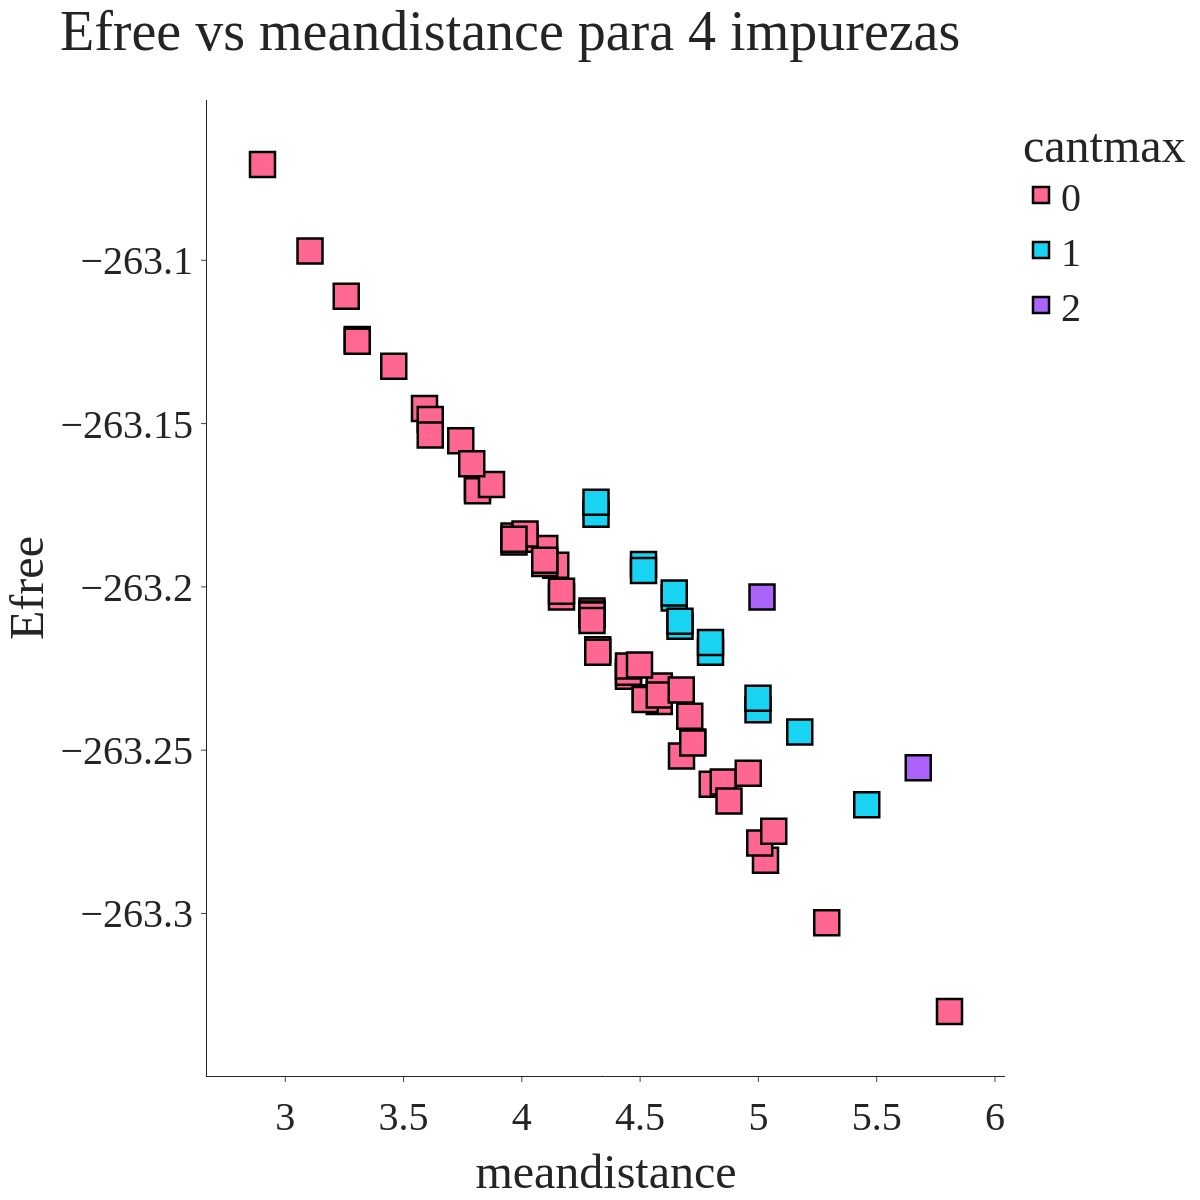
\includegraphics[width=\textwidth]{images/4_impurezas_cantmax_size10.png}
    \end{minipage}%
    \begin{minipage}[t]{0.5\textwidth}
        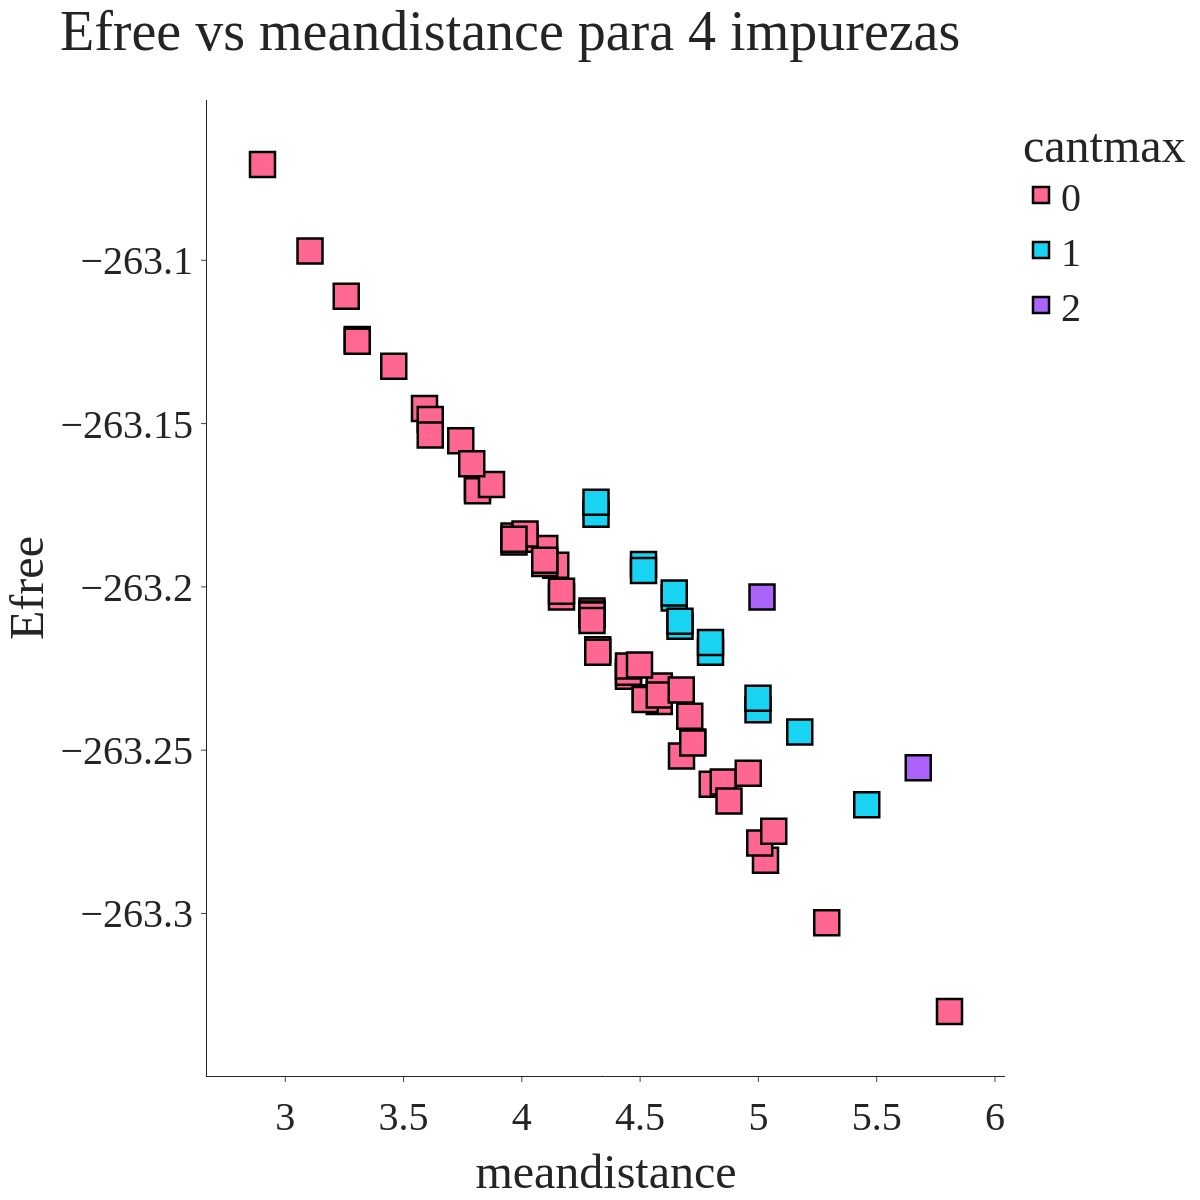
\includegraphics[width=\textwidth]{images/4_impurezas_cantmax_size10.png}    \end{minipage}%
    \caption{Ejemplo de scatterplot hecho con matplotlib.}
    \label{fig:scatterplot_3}
\end{figure}





\begin{mdframed}
    Recuerde que es imprescindible que se pueda replicar la generación de las gráficas, por lo que usted debe incluir cómo generó esos datos y  cómo podría generarlos la persona que revisa su entrega y ejecuta sus programas. Por ejemplo, si genera un scatterpolot con Tikz, usted debe explicar cómo obtener la tupla de valores que se usaron para generar la gráfica.
\end{mdframed}


\newpage
\section{Conclusiones}
\begin{mdframed}
    \textbf{La extensión máxima para esta sección es de 1 página.}
\end{mdframed}

La conclusión de su informe debe enfocarse en el resultado más importante de su trabajo. No se trata de repetir los puntos ya mencionados en el cuerpo del informe, sino de interpretar sus hallazgos desde un nivel más abstracto. En lugar de describir nuevamente lo que hizo, muestre cómo sus resultados responden a la necesidad planteada en la introducción.

\begin{itemize}
    \item  No vuelva a describir lo que ya explicó en el desarrollo del informe. En cambio, interprete sus resultados a un nivel superior, mostrando su relevancia y significado.
    \item Aunque no debe repetir la introducción, la conclusión debe mostrar hasta qué punto logró abordar el problema o necesidad planteada en el inicio. Reflexione sobre el éxito de su análisis o experimento en relación con los objetivos propuestos.
    \item No es necesario restablecer todo lo que hizo (ya lo ha explicado en las secciones anteriores). En su lugar, centre la conclusión en lo que significan sus resultados y cómo contribuyen al entendimiento del problema o tema abordado.
    \item No deben centrarse en sí mismos o en lo que hicieron durante el trabajo (por ejemplo, evitando frases como "primero hicimos esto, luego esto otro...").
    \item Lo más importante es que no se incluyan conclusiones que no se deriven directamente de los resultados obtenidos. Cada afirmación en la conclusión debe estar respaldada por el análisis o los datos presentados. Se debe evitar extraer conclusiones generales o excesivamente amplias que no puedan justificarse con los experimentos realizados.
\end{itemize}


\newpage

\section{Condiciones de entrega}
% Condiciones generales de tareas de Algoritmos y Complejidad, 20231
  \begin{itemize}
  \item
    La tarea se realizará \tcm{individualmente}
    (esto es grupos de una persona),
    sin excepciones.
  \item
    La entrega debe realizarse vía \url{http://aula.usm.cl}
    en un \tcm{tarball} en el área designada al efecto,
    en el formato \tcm{\texttt{tarea-\tnum-{rol}.tar.gz}}
    (\texttt{rol} con dígito verificador y sin guión).

    Dicho \tcm{tarball} debe contener las fuentes en \LaTeXe{}
    (al menos \tcm{\texttt{tarea-\tnum.tex}})
    de la parte escrita de su entrega,
    además de un archivo \tcm{\texttt{tarea-\tnum.pdf}},
    correspondiente a la compilación de esas fuentes.
  \item Si se utiliza algún código, idea, o contenido extraído de otra fuente, este \textbf{debe} ser citado en el lugar exacto donde se utilice, en lugar de mencionarlo al final del informe. 
  \item
    Asegúrese que todas sus entregas tengan sus datos completos:
    número de la tarea, ramo, semestre, nombre y rol.
    Puede incluirlas como comentarios en sus fuentes \LaTeX{}
    (en \TeX{} comentarios son desde \% hasta el final de la línea)
    o en posibles programas.
    Anótese como autor de los textos.
 
  %\item
  %  En la portada de su texto deberá incluir una tabla como la siguiente:
  %  
  %  \begin{center}
  %    \begin{tabular}{|l|r|}
  %      \hline
  %      \multicolumn{1}{|c|}{\textbf{Concepto}} &
  %        \multicolumn{1}{c|}{\textbf{Tiempo [min]}} \\
  %      \hline
  %      Revisión & \\
  %      \hline
  %      Desarrollo    & \\
  %      \hline
  %      Informe       & \\
  %      \hline
  %    \end{tabular}
  %  \end{center}
  %  
  %  Acá \emph{revisión} incluye revisión de apuntes,
  %  búsquedas en Internet,
  %  lectura de otras referencias;
  %  \emph{desarrollo} es el tiempo invertido en la solución pedida;
  %  \emph{informe}
  %  se refiere al tiempo requerido para confeccionar los entregables.
  \item
    Si usa material adicional al discutido en clases,
    detállelo.
    Agregue información suficiente para ubicar ese material
    (en caso de no tratarse de discusiones con compañeros de curso
     u otras personas).
\ifprograms
  \item
    Su programa ejecutable debe llamarse \tcm{\texttt{tarea\tnum}},
    de haber varias preguntas solicitando programas,
    estos deben llamarse usando el número de la pregunta,
    como \tcm{\texttt{tarea\tnum-1}},
    \tcm{\texttt{tarea\tnum-2}},
    etc.
    Si hay programas compilados, con en este caso,
    incluya una \tcm{\texttt{Makefile}}
    que efectúe las compilaciones correspondientes.

    Los programas se evalúan según que tan claros
    (bien escritos)
    son, si se compilan y ejecutan sin errores o advertencias según corresponda.
    Parte del puntaje es por ejecución correcta con casos de prueba.
    Si el programa no se ciñe a los requerimientos de entrada y salida,
    la nota respectiva es cero.
\fi    
  \item
    La entrega debe realizarse dentro del plazo indicado en \url{http://aula.usm.cl}:

    \begin{center}
        \Large{
          \textbf{NO SE ACEPTARÁN TAREAS FUERA DE PLAZO}.
        }
        \normalsize
    \end{center}
     
    
  \item
    Nos reservamos el derecho de llamar a interrogación
    sobre algunas de las tareas entregadas.
    En tal caso,
    la nota de la tarea será la obtenida en la interrogación.
    \begin{center}
      \Large{
        \textbf{NO PRESENTARSE A UN LLAMADO A INTERROGACIÓN SIN JUSTIFICACIÓN PREVIA SIGNIFICA AUTOMÁTICAMENTE NOTA 0.}
      }
    \end{center}
    
  \end{itemize}

%%% Local Variables:
%%% mode: latex
%%% ispell-local-dictionary: "spanish"
%%% End:

  
% LocalWords:  tarball tar gz pdf min entregable Makefile puntaje
% LocalWords:  Moodle

\newpage
\appendix


\section{Apédice 1}
Aquí puede agregar tablas, figuras u otro material que no se incluyó en el cuerpo principal del documento, ya que no constituyen elementos centrales de la tarea. Si desea agregar material adicional que apoye o complemente el análisis realizado, puede hacerlo en esta sección.

\begin{mdframed} 
    Esta sección es solo para material adicional. El contenido aquí no será evaluado directamente, pero puede ser útil si incluye material que será referenciado en el cuerpo del documento. Por lo tanto, asegúrese de que cualquier elemento incluido esté correctamente referenciado y justificado en el informe principal.
 \end{mdframed}


 
\printbibliography


\end{document}


